\chapter{Mathematische Methoden}
\section{Partialbruchzerlegung\label{sec:An:Partialbruch}}
Eine Funktion der Form
\begin{equation}\label{eq:Anhang:DefPolynom}
    N(z) = b_0 + b_1z + b_2z^2+ \cdots b_M z^M = \sum_{i=0}^M b_i
    z^i
\end{equation}
bezeichnen wir als Polynom M-ten Grades. Eine andere
Darstellungsform ergibt sich in der Produktdarstellung
\begin{equation}\label{eq:AnhangDefPolynomProdukt}
    N(z) = b_M (z-r_0)(z-r_1)(z-r_2)\cdots(z-r_{M-1})=b_M
    \prod_{i=0}^{M-1}(z-r_i)
\end{equation}
Dividiert man zwei Polynome so erhält man eine gebrochen rationale
Funktion\footnote{$N$ und $D$ wurden als Bezeichner für nominator
und denominator verwendet.}
\begin{equation}\label{eq:Anhang:GebrochenRational}
    P(z) = \frac{N(z)}{D(z)}
\end{equation}
Nehmen wir an, wir kennen die Produktform der jeweiligen Polynome,
so können wir unter der Bedingung, dass der Grad des Zählers
kleiner ist als der Grad des Nenners, die gebrochen rationale
Funktion auch als
\begin{equation}\label{eq:Anhang:PartialZer}
    P(z) = \frac{A_0}{z-r_0} + \frac{A_1}{z-r_1}+ \cdots \frac{A_L}{z-r_0}
\end{equation}
angeben, wobei $L$ die Ordnung des Nenners ist. Dies wird als
Partialbruchzerlegung bezeichnet. Für diese einfache Form muss
noch zusätzlich vorausgesetzt werden, dass alle Nullstellen der
Nenner-Polynoms nur einfach vorkommen. Bei Mehrfach-Nullstellen
ergibt sich eine etwas modifizierte Form der
Partialbruchzerlegung.

Die Koeffizienten der Partialbruchzerlegung können bestimmt
werden, indem der Anteil mit dem zu bestimmenden $A_i$ gekürzt
wird und die restliche Gleichung an genau $z = r_i$ berechnet
wird.
\begin{equation}\label{eq:Anhang:KoeffsPartial}
    A_i = (z-r_i)P(z)\big|_{z=r_i}
\end{equation}

Falls eine gebrochen rationale Funktion vorliegt, wo der
Zahlergrad höher ist als der Nennergrad, kann durch
Polynomdivision eine Form gefunden werden, die aus einer einfachen
Polynomfunktion mit einem zusätzlichen gebrochen rationalen Term
besteht.

\tbd{Polynomdivision, neue Form erklaeren}

Ist der Zahler- und Nennergrad gleich, wird eine Hilfsgröße
eingeführt.
\begin{equation}\label{eq:Anhang:PolyHild}
    \widehat{P}(z) = \frac{P(z)}{z}
\end{equation}


\section{komplexe Zahlen}
\subsection{Zahlendarstellung}
Komplexe Zahlen können durch zwei unterschiedliche
Beschreibungsformen dargestellt werden. Die als Rectangular
bezeichnete Form besteht aus einem Real und einem Imaginärteil,
der durch ein vor- oder nachgestelltes $i= \sqrt{-1}$ oder $j$
(ingenieursschreibweise) gekennzeichnet wird.
\begin{equation}\label{eq:KOmplexDef}
    z = x + jy
\end{equation}
Die komplexe Zahl spannt dabei eine zweidimensionale komplexe
Ebene auf. In einer Ebene lässt sich jeder Punkt aber auch durch
Polarkoordinaten darstellen. Es ist deshalb möglich komplexe
Zahlen auch in einer Polardarstellung zu verwenden.
\begin{equation}\label{eq:KomplexeZahlenPolardarstellung}
    z = r e^{j\phi}
\end{equation}
mit $e$ als Eulersche Zahl. Die Umrechnung erfolgt durch
\begin{eqnarray}\label{eq:UmrechnungPolarRect}
    r &=& \sqrt{x^2 + y^2} \\
    \phi &=& \arctan \left(\frac{y}{x} \right)\\
    x &=& r \cos (\phi)\\
    y &=& r \sin (\phi)\\
\end{eqnarray}
\subsection{Konjugation}
Als konjugierte Zahl zu einer komplexen Zahl $z$ wird bezeichnet,
wenn sich der Imaginärteil nur durch das Vorzeichen unterscheidet.
Als Symbol für den Operator zur Durchführung der Konjugation wird
$^{\ast}$ verwendet. Es gilt
\begin{equation}\label{eq:Def:Konjugation}
    (x+jy)^{\ast} = x-jy
\end{equation}

\subsection{Rechenregeln}
Für die Grundrechenarten gilt:
\begin{itemize}
    \item {\bf Addition:} Zur Addition von komplexen Zahlen werden
    die Real- und Imaginärteile separat addiert.
    \begin{eqnarray}\label{eq:Addition}
    z_3 &=& z_1 + z_2\\
     & = & (x_1 + x_2) + j (y_1 + y_2)
    \end{eqnarray}
    \item {\bf Subtraktion:} Zur Subtraktion werden
    die Real- und Imaginärteile separat subtrahiert.
    \begin{eqnarray}\label{eq:Subtraktion}
    z_3 &=& z_1 - z_2\\
     & = & (x_1 - x_2) + j (y_1 - y_2)
    \end{eqnarray}
    \item {\bf Multiplikation:} Zur Multiplikation sind zwei unterschiedliche
    Möglichkeiten vorhanden. In der Darstellung mit Real- und Imaginärteil ergibt sich.
    \begin{eqnarray}\label{eq:Multiplikation}
    z_3 &=& z_1 \cdot z_2\\
     & = & (x_1 + j y_1) (x_2 + j y_2)\\
     & = & x_1 x_2 - y_1 y_2 + j(y_1x_2 + x_1 y_2)
    \end{eqnarray}
    In der Polardarstellung ergibt sich
    \begin{eqnarray}\label{eq:Multiplikation_Polar}
    z_3 &=& r_1 e^{j\phi_1} r_2e^{j\phi_2}\\
     & = & r_1 r_2 e^{j(\phi_1+\phi_2)}
    \end{eqnarray}

    \item {\bf Division:} Zur Division ist die
    Polardarstellung besonders gut geeignet. Es ergibt sich
    \begin{eqnarray}\label{eq:Division_Polar}
    z_3 &=& \frac{r_1 e^{j\phi_1}} {r_2e^{j\phi_2}}\\
     & = & \frac{r_1} {r_2} e^{j(\phi_1-\phi_2)}
    \end{eqnarray}.
    Um eine Division in der Normalform durchzuführen, muss
    zunächst eine Erweiterung mit dem konjugiert komplexen Zähler
    erfolgen. Es ergibt sich die 3. binomische Formel, die zu
    einem rein reellwertigen Nenner führt. Eine Aufspaltung des
    Zählers in Real- und Imaginärteil ermöglicht abschließend die
    Berechnung der einzelnen Teile.
    \begin{eqnarray}\label{eq:Division}
    z_3 &=& \frac{z_1}{z_2}\\
     & = & \frac{z_1z_2^{\ast}}{z_2 z_2^{\ast}}\\
     & = & \frac{(x_1 + j y_1)(x_2 - j y_2)}{(x_2 + j y_2)(x_2 - j
     y_2)}\\
     & = & \frac{x_1x_2 + y_1y_2}{x_2^2 +
     y_2^2} + j \frac{(y_1 x_2 - x_1 y_2)}{x_2^2 +
     y_2^2}
    \end{eqnarray}
\end{itemize}
\subsection{Einige nützliche Eigenschaften und Zusammenhänge}
Aus des Grundrechenregeln und der Eigenschaft der Konjugation,
lassen sich einige nützliche Beziehungen herleiten.
    \begin{eqnarray}\label{eq:KomplexNuetzlich}
    (z_1 z_2)^{\ast} & = &  z_1^{\ast} z_2^{\ast}\\
    (z_1^{\ast} z_2)^{\ast} & = & z_1 z_2^{\ast} \\
    (z_1 + z_2)^{\ast} & = &  z_1^{\ast} + z_2^{\ast}\\
    \label{eq:Anhang:RealVonKomplex}
    z_1 + z_1^{\ast} & = & 2 \Re{z_1}\\
    \label{eq:Anhang:ImagVonKomplex}
    z_1 - z_1^{\ast} & = & 2j \Im{z_1}
    \end{eqnarray}

\subsection{Eulersche Formel}
Eine wichtige komplexe Formel ist die Eulersche Formel:
\begin{equation}\label{eq:Def:Euler}
    e^{j \omega}  = \cos(\omega) + j \sin (\omega)
\end{equation}

Daraus folgen mit (\ref{eq:Anhang:RealVonKomplex}) und
(\ref{eq:Anhang:ImagVonKomplex}) zwei nützliche Äquivalenzen:
\begin{eqnarray}
    \cos (\omega) &=& \frac{e^{j \omega} + e^{-j \omega}}{2}\\
    \sin(\omega) &=& \frac{e^{j \omega} -  e^{-j \omega}}{2j}
\end{eqnarray}

\section{Signale und ihre vektorielle Schreibweise (Besonders nützlich für Matlab)}
Die vektorielle Schreibweise von Signalen un Impulsantworten
ermöglicht es, viele Probleme der digitalen Signalverarbeitung durch
einfache lineare Algebra darzustellen und so die Lösungsansätze bzw.
mathematischen Methoden direkt anwenden zu können. Dies führt in
vielen Fällen zu einer vereinfachten Interpretation der Ergebnisse.

\subsection{Vektordarstellung}
Ein Zeitsignal $x(k)$ lässt sich als Spaltenvektor
\[
\vek{x}(k) = \left(
  \begin{array}{c}
    x(k) \\
    x(k-1) \\
    x(k-2) \\
    \vdots \\
    x(k-(N-1)) \\
  \end{array}
\right)
\]
darstellen. Häufig werden die diese Signalvektoren auch als
transponierte Zeilenvektoren eingeführt.
\[
\vek{x}(k) = [x(k) \,\, x(k-1) \,\, x(k-2) \,\, \cdots
\,\,x(k-(N-1)) ]^T
\]

Führt man dies auch für die Impulsantwort der Länge $N$ ein:
\[
    \vek{h} = [h_0 \,\, h_1 \,\, h_2 \,\, \cdots
\,\,h_{N-1} ]^T
\]
so kann ein einzelner Ausgangswert dieses Systems durch das
Skalarprodukt berechnet werden. Es gilt
\[
    y(k) = \vek{x}^T(k)\vek{h}
\]

\subsection{Vektorielle Ableitung}
\subsection{Einige spezielle Matrixdarstellungen}
Bestimmte Operatoren der digitalen Signalverarbeitung lassen sich
durch Matrix-Multiplikationen darstellen. Dies ermöglicht
Eigenschaften und Methoden der linearen Algebra direkt auf Probleme
der Signalverarbeitung anzuwenden.

\subsubsection{Faltung}

\subsubsection{Korrelation}
\subsubsection{DFT}

\subsection{Least-Squares-Lösung in Matrixform}

\section{Grundlagen der Stochastik \label{sec:Stochastik}}
Um die Grundlagen der stochastischen Signalverarbeitung zu
erläutern, sind allgemeine Kenntnisse der Stochastik und der
Statistik notwendig.

\subsection{Wahrscheinlichkeit}
Angenommen ein durchzuführendes Experiment hat einen nicht
vorhersagbaren zufälligen Ausgang, so spricht man von einem
Zufallsexperiment. Häufig sind die Möglichkeiten des Ausgangs des
Experiments abzählbar. Alle möglichen Ausgänge bilden zusammen den
Ereignisraum $\lambda$ eines Experiments. So gibt es \zB für einen
Münzwurf zwei mögliche Ausgänge; der Ereignisraum hat die beiden
Elemente {\em Kopf} oder {\em Zahl}. Beim Standard-Würfel sind
sechs Ergebnisse möglich; der Ereignisraum ist
\begin{equation}\label{eq:Bsp:EreignisraumE_Wuerfel}
    \lambda = \{1,2,3,4,5,6 \}
\end{equation}

Allgemein kann bei abzählbaren Ergebnissen der Ereignisraum durch
\begin{equation}\label{eq:BSP:EreignisraumAllg}
    \lambda = \{ \lambda_1, \lambda_2,\cdots,\lambda_N \}
\end{equation}
beschrieben werden. Interessant ist nun die Frage wie hoch ist die
Wahrscheinlichkeit $P(\lambda_k)$ der einzelnen
Elementarereignisse $\lambda_k$. Eine häufig genutzte Definition
erfolgt über die Grenzwertbetrachtung eines empirischen
Experiments. Man zählt wie oft $M_k$ ein bestimmtes
Elementarereignis $\lambda_k$ auftritt und teilt diese Anzahl
durch die Anzahl der insgesamt durchgeführten Experimente $M$.
\begin{equation}\label{eq:Def:Wahrscheinlichkeit}
    P(\lambda_k) = \lim_{M\rightarrow \infty} \frac{M_k}{M}
\end{equation}
Für den Würfel ergibt sich so das erwartetete Ergebnis, dass jede
Augenzahl genau mit der Wahrscheinlichkeit $1/6$ auftritt. Beim
Münzwurf würde sich die Wahrscheinlichkeit $1/2$ ergeben.
Entscheidend ist, die Summe über alle Wahrscheinlichkeiten aller
Elementarereignisse ergibt immer eins, da ja jedes Ergebnis des
Zufallsexperiments einem Elementarereignis zugeordnet wird.

Es gilt also:
\begin{equation}\label{eq:TotaleWahrscheinlichkeit}
    \sum_{k = 1}^{N} P(\lambda_k) = 1 \quad .
\end{equation}

Die Definition der Wahrscheinlichkeit nach Gl.
\ref{eq:Def:Wahrscheinlichkeit} ist für kontinuierliche
Ereignisräume\footnote{Zufallsvariablen, wie Sie im Abschnitt
\ref{sec:Zufallssignale} definiert wurden, gehören zu dieser
Klasse} ungeeignet, da sich für jeden konkreten Wert der
Ereignisraumes eine Wahrscheinlichkeit von Null ergeben würde.
Statt dessen wird die Wahrscheinlichkeitsfunktion $F(x)$
eingeführt, die angibt wie viele Werte kleiner als eine bestimmte
Schwelle $x$ sind. Man schreibt als Abkürzung:
\begin{equation}\label{eq:Def:Wahrscheinlichkeitsfunktion}
    F(x) = F(\lambda|\lambda<x)
\end{equation}

Für $x\rightarrow \infty$ geht diese Funktion gegen 1, da alle
Werte kleiner sind als $x = \infty$ und für $x \rightarrow
-\infty$ ist die Funktion null. Es gilt also
\begin{equation}\label{eq:WerteBereichWahrFkt}
    0 \leq F(x)\leq 1
\end{equation}

Auch für die abzählbaren Ereignisräume lässt sich die
Wahrscheinlichkeitsfunktion definieren. Es ergeben sich dann
Verläufe mit Treppenstufen. Abbildung \ref{pic:VerlaufWuerfel}
zeigt für das Beispiel des Würfels die Funktion $F(x)$.
\begin{figure}[H]
\begin{center}
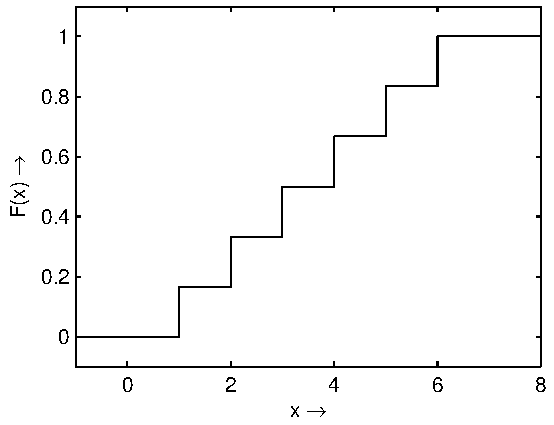
\includegraphics{psAn/FahrFunkWuerfel}
\caption{\label{pic:VerlaufWuerfel}Wahrscheinlichkeitsfunktion
$F(x)$ am Beispiel eines Standard-Würfels.}
\end{center}
\end{figure}

\subsection{Wahrscheinlichkeitsdichte\label{sec:Wahrdichte}}
Ein Äquivalent zu der Wahrscheinlichkeit bei diskreten Ereignissen
stellt die Wahrscheinlichkeitsdichtefunktion $p(x)$ für
kontinuierliche Zufallsvariablen dar. Sie ist definiert als die
Ableitung der Wahrscheinlichkeitsfunktion $F(x)$.
\begin{equation}\label{eq:Def:Wahrscheinlichkeitsdichte}
    p(x) = \frac{\delta F(x)}{\delta x}
\end{equation}
Auch für die Wahrscheinlichkeitsdichte gilt das Gesetz der totalen
Wahrscheinlichkeit.
\begin{equation}\label{eq:Def:TotaleWahrscheinlichkeit}
    \int_{-\infty}^{\infty} p(x) dx = 1
\end{equation}
Die Wahrscheinlichkeitsdichte ist außerdem nie negativ. Es gilt
\begin{equation}\label{eq:Def:Positiv}
    p(x) \geq 0
\end{equation}

Einige geläufige Beispiele für solche Wahrscheinlichkeitsdichten
oder auch Verteilungsdichten genannte Funktionen sind
gleichverteilte Zufallsgrößen in einem Interval $[a \cdots b]$
(siehe Abbildung \ref{Anh:pic:Verteilungen} links) und die
Gauss-Verteilung ((siehe Abbildung \ref{Anh:pic:Verteilungen}
rechts)), gegeben durch
\begin{equation}
    p(x) = \frac{1}{\sigma \sqrt{2\pi}} e^{-\frac{(x(k)-\mu)^2}{2\sigma^2}}
\end{equation}

\begin{figure}[H]
\begin{center}
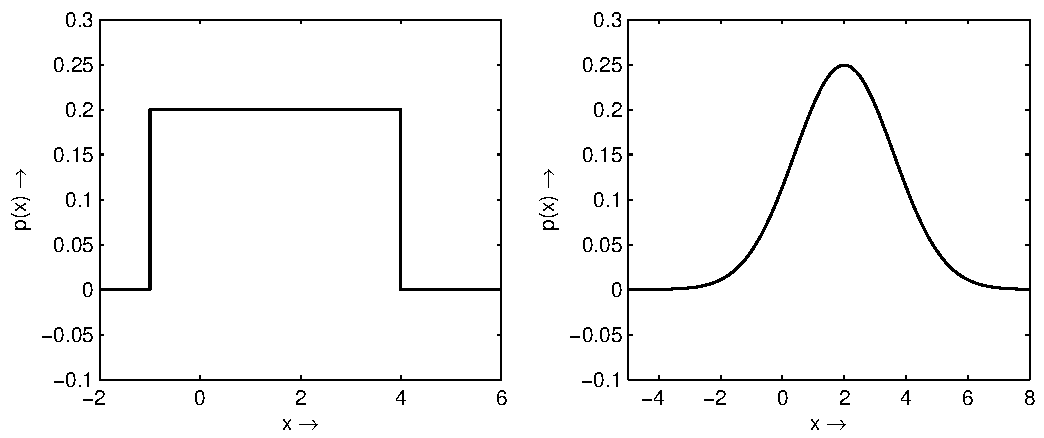
\includegraphics{psAn/VerteilGleichGauss}
\caption{\label{Anh:pic:Verteilungen}Verteilungsdichtefuntionen.
Links: Gleichverteilte Zufallsgröße im Interval $[-1 \cdots 4]$
Rechts: Gauss-verteilte Zufallsgröße mit $\mu = 1$ und $\sigma =
1.6$.}
\end{center}
\end{figure}

Zusätzlich gibt es noch weitere Verteilungsdichtefunktionen, die
bei bestimmten Anwendungen die Zufallsvariable beschreiben. Die
wichtigsten sind, die Poisson-Verteilung, die log-Normal
Verteilung, die Gamma-Verteilung, die Rayleigh-Verteilung und die
La-Place-Verteilung.

Interessant ist noch die Frage, was passiert mit den
Wahrscheinlichkeitsdichte, wenn die zugrunde liegende
Rauschprozesse addiert werden. Betrachtet man zwei gleichverteile
Zufallsgrößen mit gleichen Randparametern und addiert diese, so
erhält man eine dreiecksverteilte Größe. Eine Verknüpfung die aus
zwei rechteckigen Größen eine dreieckige Größe macht ist die
Faltung. Wir erkennen also (hier ohne Beweis), dass eine Addition
der Zufallsgrößen zu einer Faltung der Wahrscheinlichkeitsdichten
führt.
\begin{equation}\label{eq:DefZusammenhangAddundFaltung}
    y(t) = x_1(t) + x_2(t) \quad \Rightarrow \quad p(y) = p(x_1)
    \ast p(x_2)
\end{equation}

\subsection{Rechnen mit Wahrscheinlichkeiten}
Für abzählbare Ereignisräume gibt es einfach nachzuvollziehende
Rechenregeln, die sich aus der Mengenlehre ableiten.

Die Addition zweier Ereignisse ist definiert als die
Vereinigungsmenge der Einzelereignisse
\begin{equation}\label{eq:Def:AddWahrscheinlichkeiten}
    C = A + B = A \cup B = A \vee B
\end{equation}
Die Multiplikation als Schnittmenge
\begin{equation}\label{eq:Def:MultWahrscheinlichkeiten}
    C = A B = A \cap B = A \wedge B
\end{equation}
Das Kompliment $\bar{A}$ des Ereignises $A$ beinhaltet alle
Elemente eines Ereignisses, die im vollständigen Ereignisraum
$\lambda$ vorhanden sind, aber nicht im Ereignis $A$.

Weiterhin kann es nützlich sein, die Differenz im Sinne der
Mengenlehre zu definieren. Die Differenz zweier Ereignisse
beinhaltet nur die Elementarereignisse, die ausschließlich in der
ersten Menge vorkommen. Es gilt
\begin{equation}\label{eq:Def:DiffWahrscheinlichkeit}
    A-B = A\bar{B}
\end{equation}
 als die Elemente, die ausschließlich in

\begin{example}
Als Beispiel wird gerne der Würfel verwendet. Der Ereignisraum
$\lambda = \{1,2,3,4,5,6\}$. Folgende Ereignisse sollen vorliegen
können. Ereignis $A$, es ist eine gerade Zahl, also $A =
\{2,4,6\}$, und $B$ die Zahl ist kleiner oder gleich als vier,
also $B = \{1,2,3,4\}$. Dann gilt
\begin{eqnarray}
A+B &=& \{1,2,3,4,6 \}\\
A\cap B & = & \{2,4\}\\
\bar{A} &= & \{1,3,5\}\\
A-B & = & \{6 \}
\end{eqnarray}
\end{example}

\subsubsection{Bedingte Wahrscheinlichkeit und Regel von Bayes}
Eine sehr wichtige Aussage ist die Wahrscheinlichkeit eines
Ereignisses unter der Bedingung, dass vorher ein anderes Ereignis
eingetreten ist. Dies wird bedingte Wahrscheinlichkeit genannt und
durch
\begin{equation}\label{eq:Def:NameBEdingteWahr}
    P(A|B)
\end{equation}
ausgedrückt. Gelesen als die Wahrscheinlichkeit des Ereignisses
$A$ unter der Bedingung (Voraussetzung) des Ereignisses $B$.

Berechnet werden kann diese Wahrscheinlichkeit durch
\begin{equation}\label{eg:Def:BedingteWahr}
    P(A|B) = \frac{P(A B}{P(B)}
\end{equation}

\begin{example}
Es soll aus den aus den letzten Beispiel bekannten Ereignissen $A$
und $B$ die bedingte Wahrscheinlichkeit berechnet werden. Es soll
also berechnet werden, mit welcher Wahrscheinlichkeit fällt eine
gerade Augenzahl, wenn die Zahl kleiner ar vier ist.
\begin{equation}
    P(A|B) = \frac{P(AB)}{P(B)} = \frac{2/6}{4/6} = 1/2
\end{equation}
Dieses Ergebnis lässt sich auch anschaulich erklären. Durch die
Nebenbedingung, dass nur Zahlen kleiner als fünf berücksichtigt
werden sollen, stehen nur noch vier Zahlen als Ereignisraum zur
Verfügung und davon sind zwei gerade. Somit ist die
Wahrscheinlichkeit dass eine gerade Zahl vorliegt $1/2$.
\end{example}

Allgemein gilt nicht, dass $P(A|B) = P(B|A)$ ist. Für das eben
erwähnte Beispiel würde sich eine Wahrscheinlichkeit von $2/3$
ergeben, da unter den drei geraden Zahlen (Voraussetzung A), zwei
kleiner als fünf sind (Ereignis B).

Es gilt aber durch die Kommutativität der Multiplikation
\begin{equation}\label{eq:ZweiteBedingteWahr}
    P(B|A) = \frac{P(AB)}{P(A)}
\end{equation}

Durch Umstellung und Einsetzen der Gleichung
\ref{eq:ZweiteBedingteWahr} in Gleichung \ref{eg:Def:BedingteWahr}
ergibt sich der Satz von Bayes.
\begin{equation}\label{eq:Def:SatzvonBayse}
    P(A|B) = \frac{P(B|A)P(A)}{P(B)}
\end{equation}
Diese Umrechnung ermöglicht es jetzt bedingte Wahrscheinlichkeiten
zu berechnen, wenn nur die bedingte Wahrscheinlichkeit in der
anderen Richtung bekannt ist, was häufig vorkommt.

%\section{Hilbert-Transformation}
%
%\subsection{Grundlagen}
%\subsection{Rechenregeln}
%
%\subsection{Beispiele}
%\subsection{Technische Umsetzung (Design eines Hilbert-Transformators)}
